\documentclass[beamer,preview]{standalone}
\usepackage{tikz}
\usetikzlibrary{shapes,arrows,positioning,fit,backgrounds,calc,decorations.pathreplacing}
\usepackage{adjustbox}

% Define colors
\definecolor{boxblue}{RGB}{204,229,255}
\definecolor{boxborder}{RGB}{100,149,237}
\definecolor{inputyellow}{RGB}{255,243,224}
\definecolor{outputgreen}{RGB}{229,255,229}
\definecolor{arrowblue}{RGB}{70,130,180}
\definecolor{bglight}{RGB}{240,248,255}
\definecolor{titleblue}{RGB}{70,130,180}

\begin{document}
\pagestyle{empty}

\begin{adjustbox}{max totalsize={.9\textwidth}{.8\textheight},center}
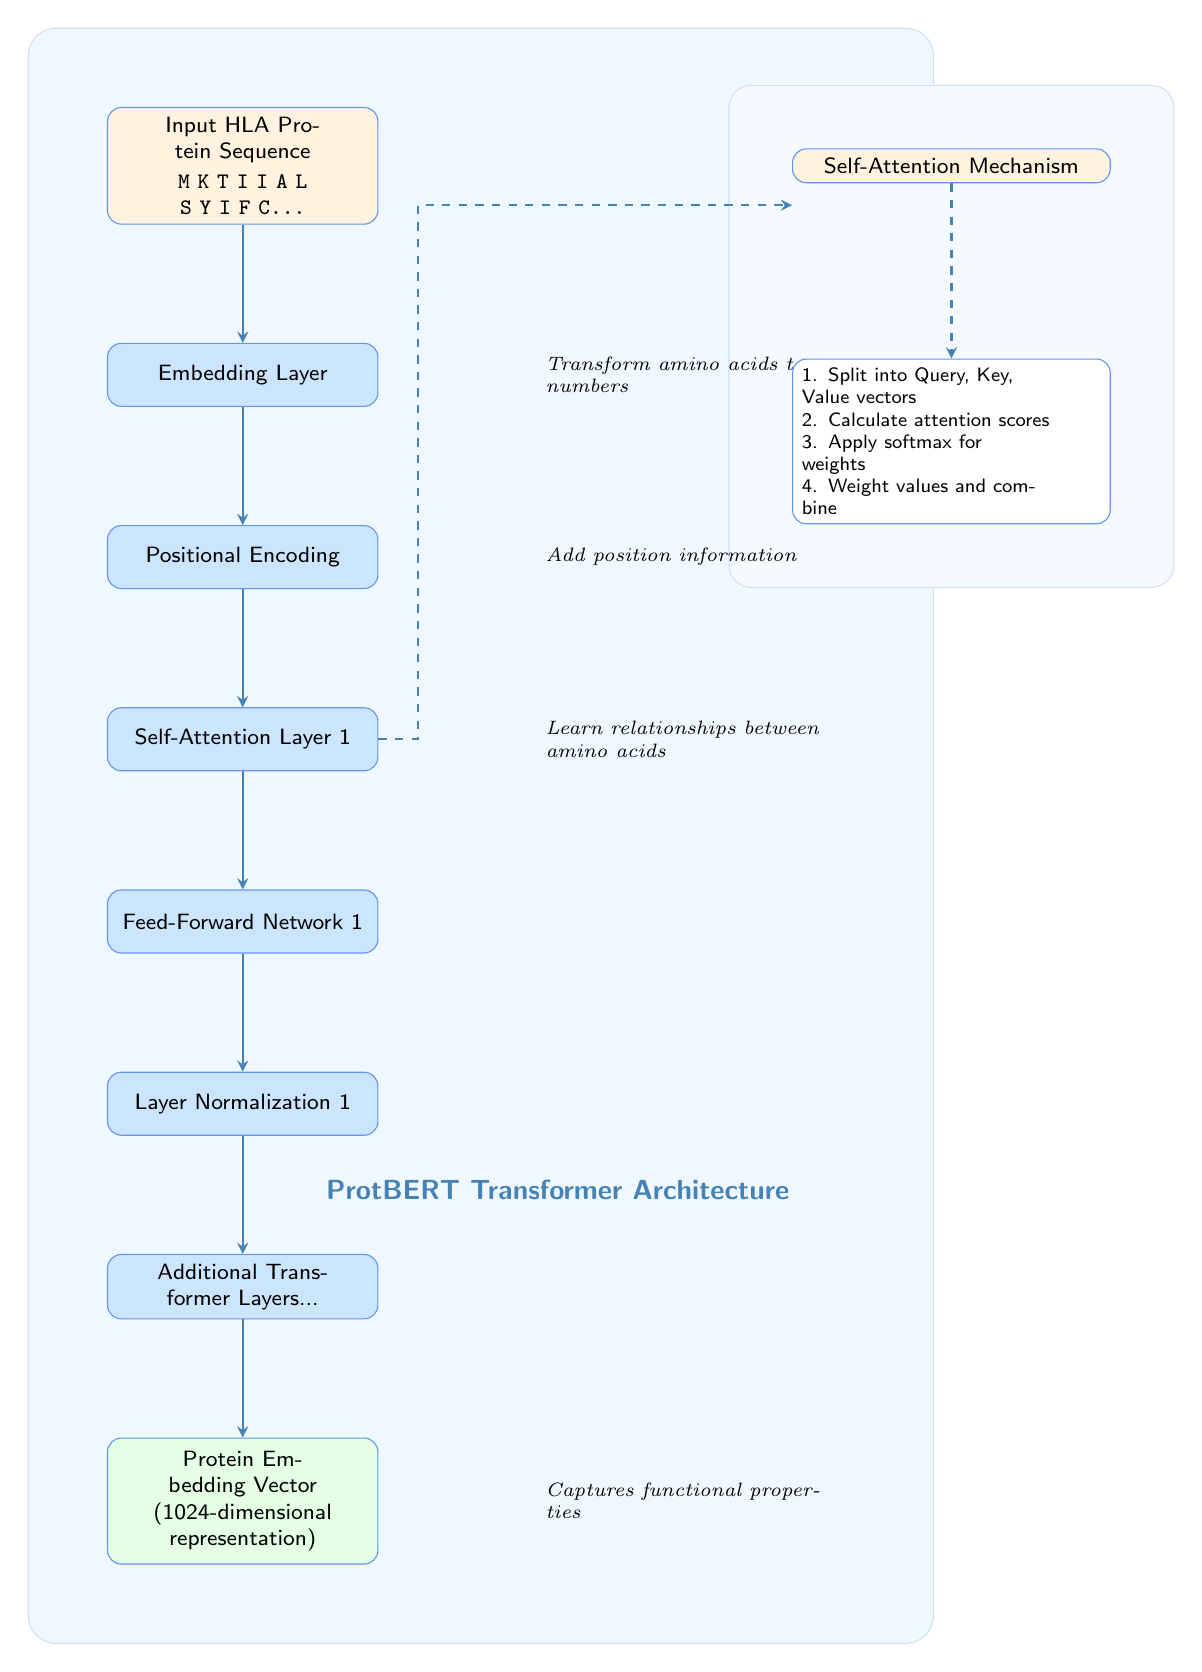
\begin{tikzpicture}[
    box/.style={draw=boxborder, rounded corners=5pt, fill=boxblue, 
                text width=3.2cm, align=center, minimum height=0.8cm, font=\sffamily\footnotesize},
    input/.style={draw=boxborder, rounded corners=5pt, fill=inputyellow, 
                 text width=3.2cm, align=center, minimum height=1.2cm, font=\sffamily\footnotesize},
    output/.style={draw=boxborder, rounded corners=5pt, fill=outputgreen, 
                  text width=3.2cm, align=center, minimum height=1.6cm, font=\sffamily\footnotesize},
    arrow/.style={thick, ->, >=stealth, arrowblue},
    note/.style={font=\scriptsize\itshape, text width=3.8cm, align=left},
    connector/.style={thick, dashed, arrowblue, ->, >=stealth},
    attention/.style={draw=boxborder, rounded corners=5pt, fill=inputyellow, 
                     align=center, text width=3.8cm, font=\sffamily\footnotesize},
    attention-detail/.style={draw=boxborder, rounded corners=5pt, fill=white, 
                           align=left, text width=3.8cm, font=\sffamily\scriptsize}
]

% Create main flow components with increased spacing
\node[input] (input) at (0,0) {Input HLA Pro-\\tein Sequence\\[0.05cm]{\ttfamily M K T I I A L\\S Y I F C...}};

\node[box, below=1.5cm of input] (embedding) {Embedding Layer};
\node[box, below=1.5cm of embedding] (pos) {Positional Encoding};
\node[box, below=1.5cm of pos] (att1) {Self-Attention Layer 1};
\node[box, below=1.5cm of att1] (ffn1) {Feed-Forward Network 1};
\node[box, below=1.5cm of ffn1] (norm1) {Layer Normalization 1};
\node[box, below=1.5cm of norm1] (more) {Additional Trans-\\former Layers...};
\node[output, below=1.5cm of more] (output) {Protein Em-\\bedding Vector\\(1024-dimensional\\representation)};

% Add explanatory notes to the right with better positioning
\node[note, anchor=west] (embedding-note) at ($(embedding.east) + (2.0,0)$) {Transform amino acids to numbers};
\node[note, anchor=west] (pos-note) at ($(pos.east) + (2.0,0)$) {Add position information};
\node[note, anchor=west] (att1-note) at ($(att1.east) + (2.0,0)$) {Learn relationships between amino acids};
\node[note, anchor=west] (output-note) at ($(output.east) + (2.0,0)$) {Captures functional properties};

% Connect main flow with arrows
\draw[arrow] (input) -- (embedding);
\draw[arrow] (embedding) -- (pos);
\draw[arrow] (pos) -- (att1);
\draw[arrow] (att1) -- (ffn1);
\draw[arrow] (ffn1) -- (norm1);
\draw[arrow] (norm1) -- (more);
\draw[arrow] (more) -- (output);

% Self-attention mechanism on right side with adjusted positioning
\node[attention] (attn) at (9,0) {Self-Attention Mechanism};

\node[attention-detail] (attn-detail) at (9,-3.5) {
    1. Split into Query, Key,\\
       Value vectors\\
    2. Calculate attention scores\\
    3. Apply softmax for\\
       weights\\
    4. Weight values and com-\\
       bine
};

% Connect attention components
\draw[connector] (attn) -- (attn-detail);

% Connect self-attention from main flow to detail with improved routing
\draw[connector] (att1.east) -- ++(0.5,0) |- ($(attn.west) + (0,-0.5)$);

% Title at bottom with adjusted position
\node[align=center, font=\normalsize\bfseries\sffamily, text=titleblue] at (4,-13) {ProtBERT Transformer Architecture};

% Create background for the main flow with increased padding
\begin{scope}[on background layer]
    \node[fill=bglight, draw=boxborder!30, rounded corners=10pt, 
          fit=(input) (embedding) (pos) (att1) (ffn1) (norm1) (more) (output) (embedding-note) (pos-note) (att1-note) (output-note),
          inner sep=1cm] (bg) {};
\end{scope}

% Create background for the attention mechanism with increased padding
\begin{scope}[on background layer]
    \node[fill=bglight!70, draw=boxborder!30, rounded corners=8pt, 
          fit=(attn) (attn-detail),
          inner sep=0.8cm] (att-bg) {};
\end{scope}

\end{tikzpicture}
\end{adjustbox}

\end{document}